\documentclass[10pt]{article}
\usepackage[margin=1in]{geometry}
\usepackage{amsmath,amssymb}
\usepackage{booktabs}
\usepackage{graphicx}
\usepackage{flafter}
\usepackage[hidelinks]{hyperref}
\usepackage[font=small,skip=4pt]{caption}
\setlength{\parindent}{0pt}
\setlength{\parskip}{0.3em}
\setlength{\abovedisplayskip}{2pt}
\setlength{\belowdisplayskip}{2pt}
\setlength{\textfloatsep}{8pt}
\setlength{\intextsep}{6pt}
\usepackage{titlesec}
\titlespacing*{\section}{0pt}{0.5em}{0.15em}

\title{\vspace{-2.2em}Whack-a-mole Learning for Implied Volatility Calibration:\\
\large A PyTorch Implementation, a Test of Its PDE Loss, and a Stabilized Update\vspace{-0.4em}}
\author{Bjorn Thor Stefansson \quad CEE 292 \quad \small\url{https://github.com/bjornts/waml-implied-volatility}\vspace{-0.6em}}
\date{}

\begin{document}
\maketitle
\vspace{-2.4em}

\section{Introduction}
Options are quoted by price, but they are usually compared through implied volatility (IV): the volatility that makes the Black--Scholes formula match the price. Plotting IV against strike and maturity gives a surface. We only see quotes at some points, so we have to fill in the rest. Not every fit will do, because some shapes would allow risk-free profit, known as arbitrage.

Hoshisashi, Phelan and Barucca~\cite{waml} fill in the surface with a neural network trained on three goals: match the quotes, satisfy a pricing PDE, and avoid arbitrage. These goals compete, so they also propose Whack-a-mole Learning (WamL), which changes the weight of each goal during training.

I implemented this method in PyTorch, using the lead author's public JAX notebook~\cite{notebook} only for settings the paper leaves out, and asked what each part contributes. The PDE loss turns out to add nothing, because it cancels algebraically. The no-arbitrage penalties do the useful work. WamL's weight update, as written, made every run lose its fit. My enhancement, a one-line change to that update, prevents most of these failures.

\section{Method}
We need a surface we can read at any strike $K$ and maturity $\tau$, so I use a neural network that outputs a positive IV, $\varphi_\theta(K,\tau)$ (4 hidden layers of 64 units, tanh, softplus output). Quotes are prices, so Black--Scholes turns this IV into a price we can compare with them: $\Phi_\theta=C_{\mathrm{BS}}(K,\tau,\varphi_\theta)$. These prices meet the boundary conditions for any positive volatility, so I need no boundary loss.

Matching quotes is not enough, so the prices must also obey two kinds of rule. The first is Dupire's PDE, $f=0$ in~\eqref{eq:constraints}, which uses a local volatility $\sigma_{\mathrm{LV}}$ computed from the IV network through~\eqref{eq:lv}. The second is the set of Carr--Madan no-arbitrage rules~\cite{carr}, the inequalities in~\eqref{eq:constraints}:
\begin{equation}
  f := \frac{\partial C}{\partial \tau}+rK\frac{\partial C}{\partial K}-\frac12\sigma_{\mathrm{LV}}^2K^2\frac{\partial^2 C}{\partial K^2}=0,
  \qquad
  -e^{-r\tau}\le\frac{\partial C}{\partial K}\le 0,\quad
  \frac{\partial^2 C}{\partial K^2}\ge 0,\quad
  \frac{\partial C}{\partial \tau}\ge 0,
  \label{eq:constraints}
\end{equation}
\begin{equation}
  \sigma_{\mathrm{LV}}^2=\frac{A}{B},\qquad A=\sigma^2+2\sigma\tau\left(\sigma_\tau+rK\sigma_K\right),\quad
  B=1+2d_+K\sqrt{\tau}\,\sigma_K+K^2\tau\left(d_+d_-\sigma_K^2+\sigma\sigma_{KK}\right).
  \label{eq:lv}
\end{equation}

Each rule becomes a term in the loss, next to the quote fit: $\mathcal{L}=\sum_\beta\lambda_\beta\hat{\mathcal L}_\beta$, with $\hat{\mathcal L}_\beta=N_\beta^{-1}\sum_j m_\beta^{(j)}\big(r_\beta^{(j)}\big)^2$. Here $r_\beta^{(j)}$ is the error at point $j$, which is zero for an inequality that holds. These terms can differ in size by many orders of magnitude, so fixed weights can let one term dominate. WamL therefore changes the weights every 100 steps. Per-point weights $m$ grow where the error is large~\cite{sapinn}, and each loss weight $\lambda$ grows when its term's gradient is small compared with the others~\cite{expert}:
\begin{equation}
  m_\beta^{(j)}\leftarrow m_\beta^{(j)}+\eta_m\,\partial\hat{\mathcal L}_\beta/\partial m_\beta^{(j)},
  \qquad
  \lambda_\beta\leftarrow\tfrac12\Big(\lambda_\beta+\sum\nolimits_{\beta'}\big|\nabla_\theta\hat{\mathcal L}_{\beta'}\big|\,\big/\,\big|\nabla_\theta\hat{\mathcal L}_{\beta}\big|\Big).
  \label{eq:waml}
\end{equation}
If a gradient is exactly zero, the paper resets that weight to 1, a detail that matters later.

To judge a fitted surface we need to know the true one, and for a real market we never do. I therefore use synthetic data: I pick a true surface with Hagan's SABR formula~\cite{sabr} and the paper's parameters, then generate quotes from it. The paper leaves out the interest rate and noise level, and its quote locations come from private S\&P 500 data, so I take these from the notebook ($r=0.05$, $10\%$ noise on volatility). Real quotes can be noisy or scarce, so I test three cases: clean (300 quotes), noisy (300 quotes with noise) and sparse (50 quotes). Each case uses five seeds, because one run can mislead. Training follows the paper (10,000 Adam steps, up to about 55 min per run), except for weight decay, whose value it does not give.

To see what each part adds, I add the parts one at a time, giving four models. A \textbf{data-only} network just fits the quotes. A \textbf{PINN} adds the PDE loss. A derivative-constrained PINN (\textbf{DCPINN}) also adds the no-arbitrage penalties. These three use fixed weights, and \textbf{WamL} then lets the weights change. I score each model on 2,000 noiseless points it never saw in training, using price error and IV error. IV error skips the $9\%$ of points with vega below $10^{-3}$, where the price barely depends on volatility. To measure arbitrage, I count the share of a $201\times201$ grid that breaks the rules in~\eqref{eq:constraints}.

\section{Why the PDE loss cancels}
\label{sec:residual}
The PDE loss is the physics in this model, so we would expect it to keep the surface realistic. To see whether it can, we put the network's price into $f$. Write $C=C_{\mathrm{BS}}(K,\tau,\sigma(K,\tau))$ with $\sigma=\varphi_\theta$ and vega $V=\partial_\sigma C_{\mathrm{BS}}$, where subscripts on $C$ and $\sigma$ mean derivatives along the surface. Two facts about Black--Scholes at fixed volatility make this easy: it satisfies Dupire's PDE, and its second derivatives are multiples of vega:
\begin{equation}
  \partial_\tau C_{\mathrm{BS}}+rK\partial_K C_{\mathrm{BS}}=\tfrac12\sigma^2K^2\partial_{KK}C_{\mathrm{BS}},\;
  \partial_{KK}C_{\mathrm{BS}}=\frac{V}{K^2\sigma\tau},\;
  \partial_{K\sigma}C_{\mathrm{BS}}=\frac{Vd_+}{K\sigma\sqrt{\tau}},\;
  \partial_{\sigma\sigma}C_{\mathrm{BS}}=\frac{Vd_+d_-}{\sigma}.
  \label{eq:identities}
\end{equation}
Now apply the chain rule to $C$ and use~\eqref{eq:identities}. Both parts of $f$ become a common factor times $A$ or $B$ from~\eqref{eq:lv}:
\begin{align}
  C_\tau+rKC_K&=\tfrac12\sigma^2K^2\partial_{KK}C_{\mathrm{BS}}+V(\sigma_\tau+rK\sigma_K)=\frac{V}{2\sigma\tau}A,\label{eq:left}\\
  \tfrac12K^2C_{KK}&=\tfrac12K^2\big(\partial_{KK}C_{\mathrm{BS}}+2\sigma_K\partial_{K\sigma}C_{\mathrm{BS}}+\sigma_K^2\partial_{\sigma\sigma}C_{\mathrm{BS}}+V\sigma_{KK}\big)=\frac{V}{2\sigma\tau}B.\label{eq:right}
\end{align}
Since $\sigma_{\mathrm{LV}}^2=A/B$, putting~\eqref{eq:left} and~\eqref{eq:right} into $f$ cancels everything wherever $B\neq0$:
\begin{equation}
  f=\frac{V}{2\sigma\tau}A-\frac{A}{B}\cdot\frac{V}{2\sigma\tau}B=0.
  \label{eq:cancel}
\end{equation}
The network's weights never entered this calculation, so $f=0$ for any smooth positive network, trained or not. This makes sense: \eqref{eq:lv} comes from solving $f=0$ for $\sigma_{\mathrm{LV}}^2$, and the loss just puts that answer back in. So this loss cannot push the network toward any particular surface. The author's notebook computes local volatility the same way, and the paper does not discuss this.

A direct measurement agrees. Using automatic differentiation on an untrained $4\times16$ network in single precision, mean $f^2$ is already $3\times10^{-14}$, far below the $1\times10^{-3}$ of mean $C_\tau^2$. After training on prices alone, without the PDE loss, it is $1\times10^{-15}$. In double precision, both values fall below $10^{-30}$. The residual therefore measures rounding, not training, so adding this loss should change nothing. Training can test this.

\section{Results and discussion}
\label{sec:results}
Table~\ref{tab:results} and Figure~\ref{fig:results} show the results, which I go through in the order the parts were added. First comes the PDE loss. As predicted, it changes almost nothing in double precision: on noisy data, the PINN and the data-only network agree to three decimals in IV error on every seed, with median violations of $19.07\%$ and $19.08\%$. Single precision looks different at first, because the PINN cuts violations from $18.50\%$ to $0.51\%$. But the loss is mathematically zero and the gain disappears when rounding shrinks, so the gain most likely comes from rounding noise, not from the PDE. So a low residual does not show that a surface obeys the physics.

If the PDE loss is not shaping the surface, the no-arbitrage penalties must be. In double precision they cut violations on noisy data from about $19\%$ to $0.26\%$, and IV error from $0.021$ to $0.013$. One of the 20 DCPINN runs did lose its fit, but this is still a good baseline.

\begin{table}[t]
\centering\footnotesize\setlength{\tabcolsep}{2.6pt}
\caption{Held-out IV error and violations (Viol., medians of five seeds), and collapsed runs (Coll.): final quote MSE above $10^{-4}$, about what a flat surface achieves, and over 10 times the run's best. Price errors follow the same pattern.}
\label{tab:results}
\begin{tabular}{lcccccccccccc}
\toprule
 & \multicolumn{3}{c}{Noisy, single} & \multicolumn{3}{c}{Noisy, double} & \multicolumn{3}{c}{Clean, single} & \multicolumn{3}{c}{Sparse, single}\\
\cmidrule(lr){2-4}\cmidrule(lr){5-7}\cmidrule(lr){8-10}\cmidrule(lr){11-13}
Model & IV & Viol.\,\% & Coll. & IV & Viol.\,\% & Coll. & IV & Viol.\,\% & Coll. & IV & Viol.\,\% & Coll.\\
\midrule
Data-only & 0.021 & 18.50 & 0/5 & 0.021 & 19.08 & 0/5 & 0.008 & 0.00 & 0/5 & 0.010 & 9.39 & 0/5\\
PINN & 0.020 & 0.51 & 0/5 & 0.021 & 19.07 & 0/5 & 0.008 & 0.00 & 0/5 & 0.010 & 9.47 & 0/5\\
DCPINN & 0.019 & 0.10 & 1/5 & 0.013 & 0.26 & 0/5 & 0.008 & 0.00 & 0/5 & 0.010 & 0.00 & 0/5\\
WamL, paper's rule & 0.247 & 0.00 & 5/5 & 1.053 & 54.84 & 5/5 & 0.222 & 0.00 & 5/5 & 1.889 & 0.00 & 5/5\\
WamL, no PDE loss & 0.045 & 0.00 & 2/5 & 0.484 & 29.98 & 5/5 & 0.318 & 27.40 & 3/5 & 0.073 & 0.00 & 3/5\\
WamL, gradient floor & 0.015 & 0.29 & 1/5 & 0.023 & 0.00 & 0/5 & 0.008 & 0.00 & 0/5 & 0.010 & 0.00 & 0/5\\
\bottomrule
\end{tabular}

\end{table}

\begin{figure}[t]
\centering
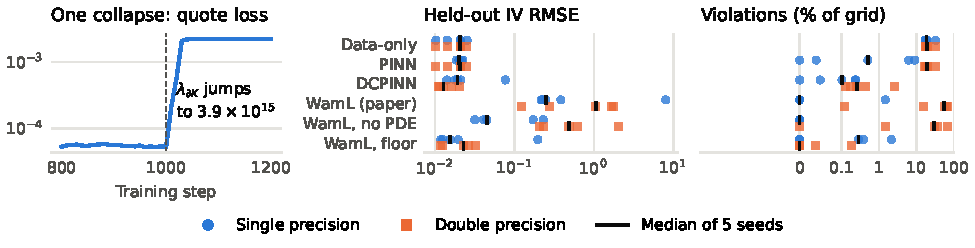
\includegraphics[width=\textwidth]{figures/results.pdf}
\caption{Left: a collapse in one noisy single-precision run (seed 4, paper's rule). Center and right: noisy case, with one dot per seed. Few violations on a collapsed surface is not a success, because it no longer fits the quotes.}
\label{fig:results}
\end{figure}

WamL should improve on this baseline by choosing better weights. With the paper's rule it did the opposite: all 20 runs collapsed, meaning they fit well at first and then suddenly lost the fit. The left panel of Figure~\ref{fig:results} shows this happening in one run. At step 1,000, a no-arbitrage loss of $2.6\times10^{-24}$ has a very small gradient that is not exactly zero. The reset therefore does not apply, and~\eqref{eq:waml} raises that loss weight from 1 to $3.9\times10^{15}$. Within 30 steps the quote loss rises about 40-fold, and it never recovers.

One run does not prove the cause, so I checked the other explanations. Is it the PDE term? No: without it, 8 of 15 single-precision runs and all 5 double-precision runs still collapsed, because the no-arbitrage terms also have very small gradients once they are nearly satisfied. Is it rounding alone? No: double precision collapsed too, with weights above $10^{30}$ on seed 4. Is it the per-point weights? They barely moved. That leaves the loss-weight update as the most likely cause. I did not run the authors' code and my setup differs from the paper's, so this shows the rule is unstable in my setting, not that the published results are wrong.

If near-zero gradients are the trigger, the fix follows: treat a negligibly small gradient like a zero one. My \textbf{gradient floor} resets a loss weight to 1 whenever $|\nabla_\theta\hat{\mathcal L}_\beta|\le\epsilon\sum_{\beta'}|\nabla_\theta\hat{\mathcal L}_{\beta'}|$, which keeps every weight below $1/\epsilon$. In the code, this changes one condition in \texttt{update\_balance\_weights}: \mbox{\texttt{scale == 0}} becomes \mbox{\texttt{scale <= floor * total}}. I set $\epsilon=10^{-3}$ before seeing any results, so it is not tuned to the test data, and removed the PDE loss, which adds nothing.

The floor works well, but not perfectly. In single precision, 14 of 15 runs avoided collapse, against 7 of 15 for the same loss without the floor. In double precision, all 5 runs avoided it, against none without the floor. Accuracy is close to fixed-weight DCPINN: IV error is similar in single precision, and in double precision the floor has fewer violations ($0.00\%$ vs.\ $0.26\%$) but higher IV error ($0.023$ vs.\ $0.013$). One run still collapsed: noisy seed 2 in single precision fit well until step 9,500 and then lost its fit (IV error $0.197$), even though its weights stayed below 1,000. The floor therefore lowers the risk of collapse but does not remove it.

\section{Conclusion}
What does each part contribute? The PDE loss, as formulated, cancels algebraically and adds no constraint. The no-arbitrage penalties do the work of removing arbitrage. WamL's weight update, as written, collapsed all 20 runs in my tests, and a one-line gradient floor lets 19 of 20 avoid this. Even then it did not clearly beat fixed weights, so I found no evidence here that adaptive weights help. Two next steps follow: a separate local-volatility network, so that $f$ no longer cancels, and hard no-arbitrage constraints.

{\footnotesize
\begin{thebibliography}{9}\setlength{\itemsep}{0pt}\setlength{\parskip}{0pt}
\bibitem{waml} K.~Hoshisashi, C.~E.~Phelan, P.~Barucca. Whack-a-mole Learning: Physics-Informed Deep Calibration for Implied Volatility Surface. \emph{IEEE CIFEr}, 2024. \href{https://doi.org/10.1109/CIFER62890.2024.10772909}{doi:10.1109/CIFER62890.2024.10772909}.
\bibitem{notebook} K.~Hoshisashi. DC-PINNs notebook. \url{https://github.com/khoshisashi/DC-PINNs}.
\bibitem{carr} P.~Carr, D.~B.~Madan. A note on sufficient conditions for no arbitrage. \emph{Finance Research Letters} 2(3), 2005.
\bibitem{sapinn} L.~McClenny, U.~Braga-Neto. Self-adaptive PINNs using a soft attention mechanism. arXiv:2009.04544, 2020.
\bibitem{expert} S.~Wang, S.~Sankaran, H.~Wang, P.~Perdikaris. An expert's guide to training PINNs. arXiv:2308.08468, 2023.
\bibitem{sabr} P.~S.~Hagan, D.~Kumar, A.~S.~Lesniewski, D.~E.~Woodward. Managing smile risk. \emph{Wilmott}, 2002.
\end{thebibliography}
}
\end{document}
